\documentclass[tikz,border=1pt]{standalone}
\usetikzlibrary{intersections}
\begin{document}
	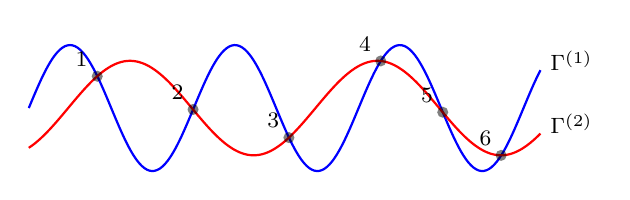
\begin{tikzpicture}
		
		% two curves
		\draw[thick,smooth,samples=200,color=blue,domain=0:6.5,name path=gamma1] plot (\x,{0.8*sin(3*\x r)});
		\draw[thick,smooth,samples=200,color=red,domain=0:6.5,name path=gamma2] plot (\x,{0.6*sin((2*\x-1) r)});
				
		% notations
		\draw (6.5, 0.6) node [right] {\footnotesize$\Gamma^{(1)}$};
		\draw (6.5, -0.2) node [right] {\footnotesize$\Gamma^{(2)}$};
		
		\fill [name intersections={of=gamma1 and gamma2,name=i,total=\t}]
			  [black,opacity=0.5,every node/.style={above left,black,opacity=1}]
			  \foreach \s in {1,...,\t}{(i-\s) circle (2pt) node {\footnotesize\s}};
	\end{tikzpicture}
\end{document}